\documentclass[20pt,margin=1in,innermargin=-4.5in,blockverticalspace=-0.25in]{tikzposter}
\geometry{paperwidth=40in,paperheight=30in}
\usepackage[utf8]{inputenc}
\usepackage{amsmath}
\usepackage{amsfonts}
\usepackage{amsthm}
\usepackage{amssymb}
\usepackage{mathrsfs}
\usepackage{graphicx}
\usepackage{adjustbox}
\usepackage{enumitem}

\renewcommand{\algorithmiccomment}[1]{$/\!/$ \parbox[t]{4.5cm}{\raggedright #1}}
\usepackage[noend]{algorithmic}

\newcommand{\TITLE}[1]{\item[#1]}
\renewcommand{\algorithmiccomment}[1]{$/\!/$ \parbox[t]{4.5cm}{\raggedright #1}}
% ugly hack for for/while
\newbox\fixbox
\renewcommand{\algorithmicdo}{\setbox\fixbox\hbox{\ {} }\hskip-\wd\fixbox}
% end of hack
\newcommand{\algcost}[2]{\strut\hfill\makebox[1.5cm][l]{#1}\makebox[4cm][l]{#2}}
\usepackage[backend=biber,style=numeric]{biblatex}
\usepackage{emory-theme}

\usepackage{mwe} % for placeholder images

\addbibresource{refs.bib}

% set theme parameters
\tikzposterlatexaffectionproofoff
\usetheme{EmoryTheme}
\usecolorstyle{EmoryStyle}

\title{Calculator for sinhx}
\author{Xueying Li}
\titlegraphic{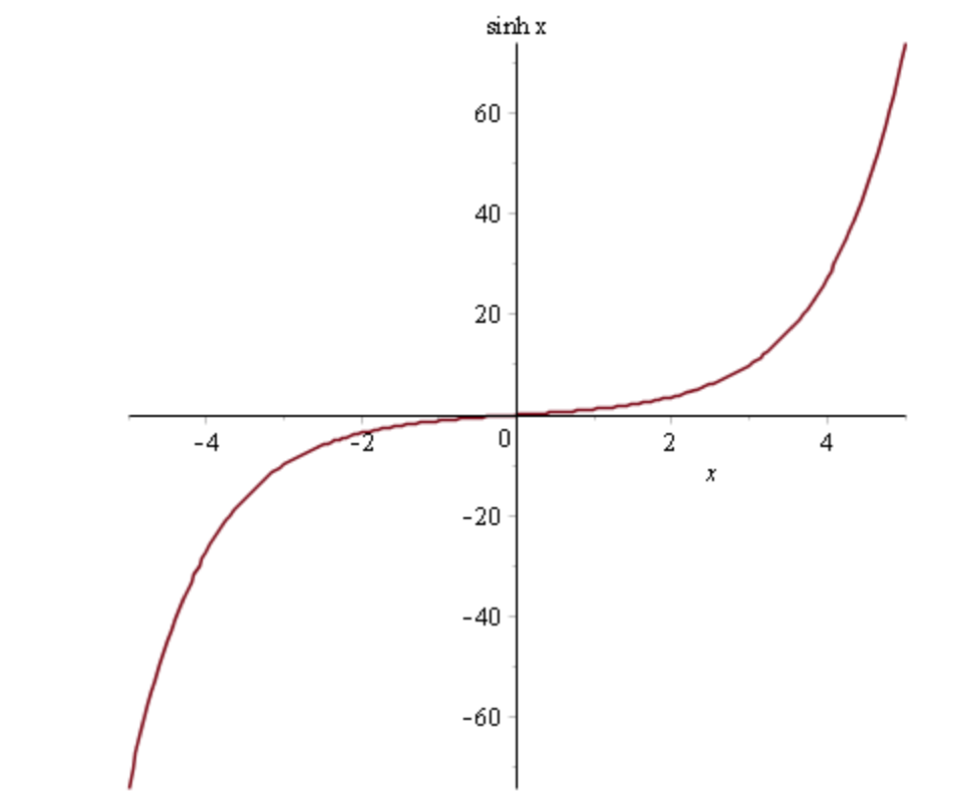
\includegraphics[width=0.09\textwidth]{sinhx.png}}

% begin document
\begin{document}
\maketitle
\centering
\begin{columns}
\column{0.32}
    \block{Function}{
    asdf   $ \sinh x\ $is a transcendental function and it is defined as following(Formula 1).

    \begin{align*}
    F3:  \sinh x = \frac{e^{x}-e^{-x}}{2}\label{eq:1}
    \end{align*}
    
    asdf  e $ \e^{x}\ $is expanded to Taylor Series.
    \begin{align*}
    \sum_{n=0}^{\infty } \frac{x^{n}}{n!}= \frac{x^{0}}{0!} + \frac{x^{1}}{1!} + \frac{x^{2}}{2!}+\frac{x^{3}}{3!}+...
    \end{align*}

    }
    \block{Algorithms}{

          asdf   Following gives the Algorithms[1-3].
          \begin{tikzfigure}[Algorithm for sinhx]
           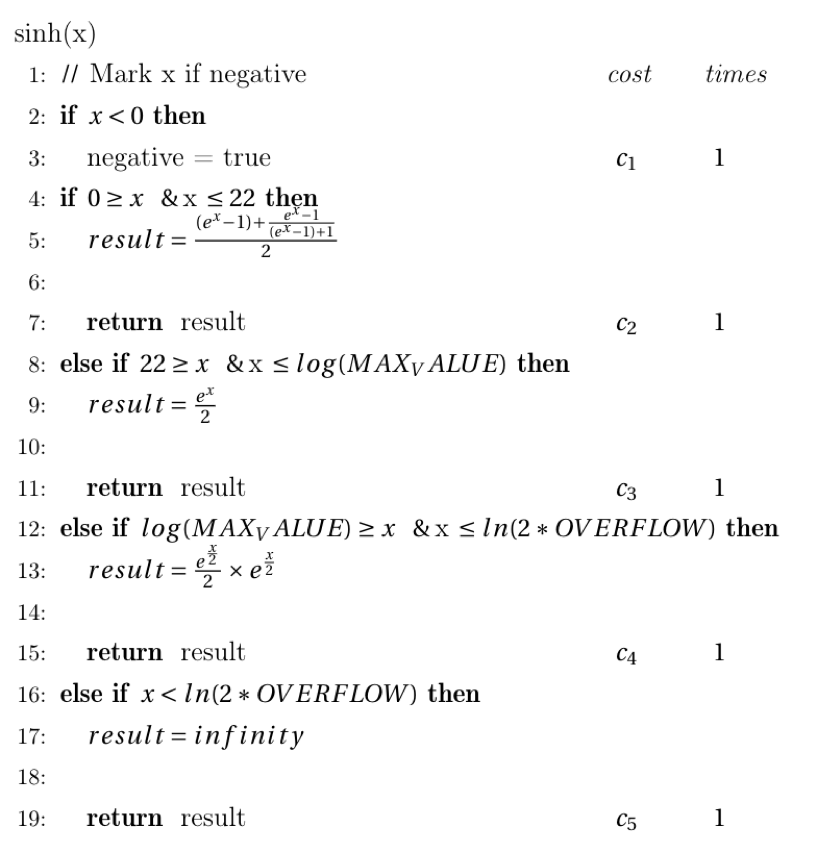
\includegraphics[width=0.7\linewidth]{algorithm1.png}
          \end{tikzfigure}
          
          \begin{tikzfigure}[Algorithm for Expansion]
           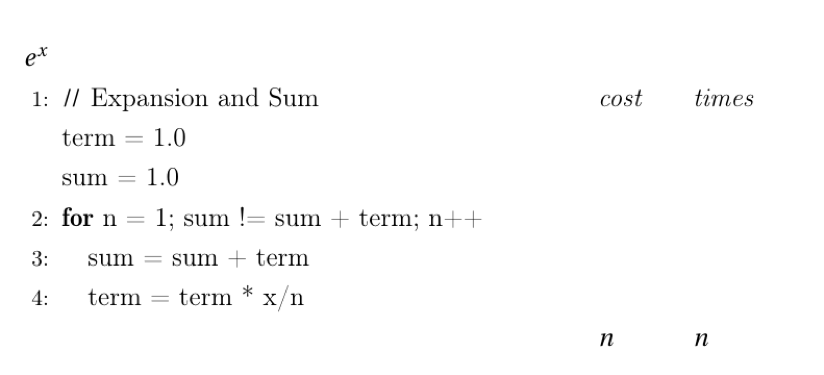
\includegraphics[width=0.7\linewidth]{e.png}
          \end{tikzfigure}
          
    }
    \column{0.36}
    \block{User Interface}{
        User Interface(UI) is designed as Text-Based User Interface(TUI).Figure 3 shows typical messages(Msgs) from TUI of the calculator application. Each Msg is related to a requirement regarding to UI.  Model-View-Controller(MVC) design pattern is implemented to decrease coupling and increase cohesion[4]. a class diagram is shown as following(figure 4).\\
        
        
        \vspace{1em}
        \begin{tikzfigure}[Texical User Interface]
           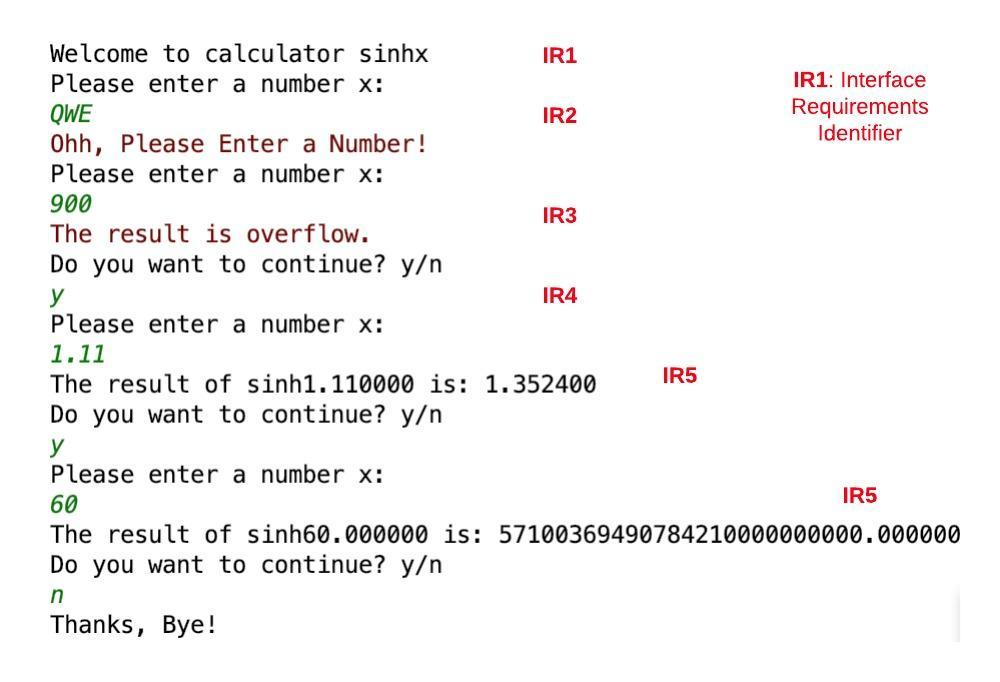
\includegraphics[width=0.75\linewidth]{UIImplementation.jpeg}
        \end{tikzfigure}
        
        \vspace{1em}
        \begin{tikzfigure}[Class Diagram]
           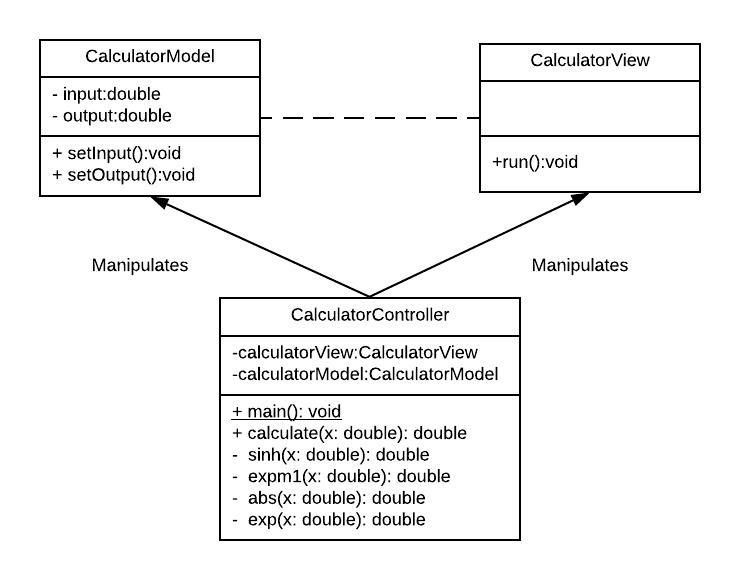
\includegraphics[width=0.65\linewidth]{UIDesign.jpeg}
        \end{tikzfigure}
        
    }

    \column{0.32}
    \block{Test and Review}{
        Following gives the report of source code review result and test result.
        \begin{tikzfigure}[Source code review result]
            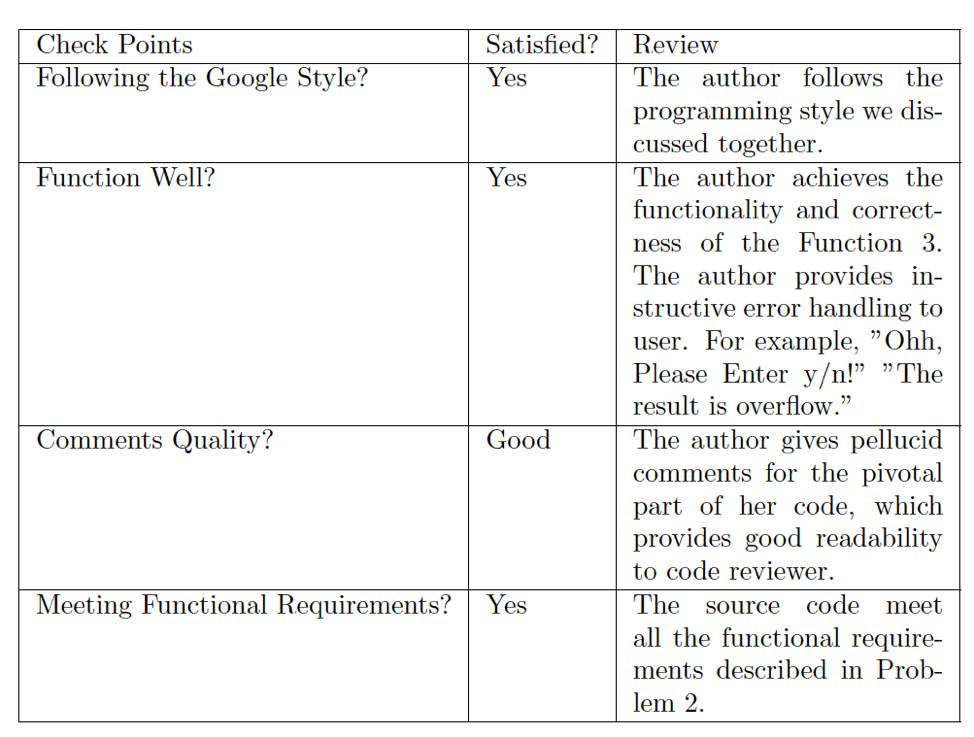
\includegraphics[width=0.7\linewidth]{review.png}
        \end{tikzfigure}
        
        
        \begin{tikzfigure}[Test Result]
            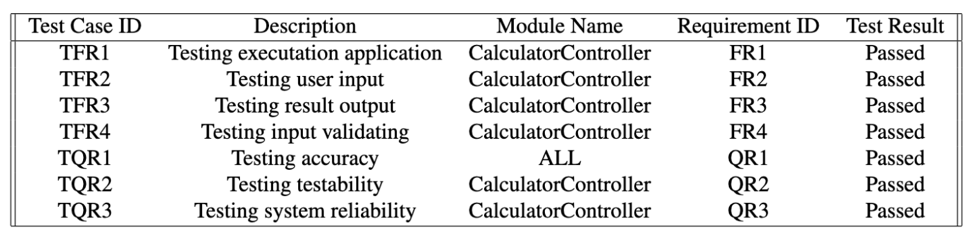
\includegraphics[width=0.7\linewidth]{test.png}
        \end{tikzfigure}
    }
    
    
    \block{References}{
       \begin{thebibliography}{3}
    \bibitem{1}
mathcentre, Universities of Loughborough \\
\textit{http://www.mathcentre.ac.uk/resources/workbooks/mathcentre/hyperbolicfunctions}

\bibitem{2}
Feldt R 
\textit{re_lecture5b_100914, unpublished}

\bibitem{3}
Source for java.lang.StrictMath
\textit{http://developer.classpath.org/doc/java/lang/StrictMath-source.html}

\bibitem{4}
Robert M. Kline, 
\textit{https://www.cs.wcupa.edu/rkline/java/mvc-design.html}

\end{thebibliography}
    }
\end{columns}
\end{document}